


\documentclass[a4paper,12pt]{article}
\usepackage{graphicx}
\usepackage{tabularx}  % Add to preamble
\usepackage{array}
\usepackage{float}
\usepackage[backend=biber,style=numeric]{biblatex}
\addbibresource{references.bib}




% title
\title{Optimization of Plant Growth on Urban Terraces Using Embedded Devices}
\author{ultraego4 \\
	\small company \\
	\small \texttt{email}}
\date{\today}

\begin{document}



\maketitle

\newpage

\begin{abstract}
	This paper explores the optimization of plant growth on urban terraces using embedded devices. The study employs various sensors and automation systems to monitor and improve environmental factors such as temperature, light and soil moisture. The goal is to enhance plant health and maximize growth in constrained urban spaces. TODO rewrite this
\end{abstract}

\newpage

\tableofcontents

\newpage

\section{TODO Research topics and explanations}

\begin{itemize}
\item why certain seeds were chosen and why are they not original $\rightarrow$ were not available
\item explain the environment you developed your code in $\rightarrow$ esp-idf, clang etc.
\item list all aliexpress items with links and detailed information
\item what soil and why it has been chosen $\rightarrow$ really nothing were available
\item picture on the soil, seeds, brand fully analyzed where it comes from $\rightarrow$ also do the same for the soil
\item explain the problem of getting the correct npk value and the dilemma of bio plants $\rightarrow$ research natural ways to fulfill the npk needs
\item pictures of the environment aka the the TERRACE
\item explain why do all of this in the first place ? :)))
\item natural npk can be reached with natural things
\begin{itemize}
	\item{how do you determine the ratio, what website to use or research paper to see whats the correct npk for each plants}
	\item{how much you give from that natural fertilizer, one spoon or what?}
	\item{each natural npk material has ?/gram nutrient?}
	\item{the soil i bought contains how much npk and ph??}
\end{itemize}
\item explain why leave space between plants in the seedling and full blown phase
\end{itemize}






\section{Climate meter circuit}

\section{Seeds}
\subsection{Tomato (Solanum lycopersicum)}


\begin{table}[H]
	\centering
	\begin{tabularx}{\textwidth}{|>{\centering\arraybackslash}p{4cm}|>{\centering\arraybackslash}p{4cm}|>{\centering\arraybackslash}p{5cm}|}
		\hline
		\textbf{Parameter} & \textbf{Value} & \textbf{Remarks} \\
		\hline
		Growing period & 90–150 days & From transplanting to harvest \\
		\hline
		Optimal temperature & 18–25°C (day), 10–20°C (night) & Above 25°C with high humidity reduces yield \\
		\hline
		Soil preference & pH 5–7 & Well-drained light loam; avoid water logging \\
		\hline
		Nitrogen ($m/m\%$) & 100–150 kg/ha & For high-yielding varieties \\
		\hline
		Phosphorus pentoxide ($m/m\%$) & 65–110 kg/ha & For high-yielding varieties \\
		\hline
		Potassium oxide ($m/m\%$) & 160–240 kg/ha & For high-yielding varieties \\
		\hline
		Humidity tolerance & Low & High humidity increases disease risk \\
		\hline
		Sensitivity to salinity & Moderate & Germination phase is most sensitive \\
		\hline
		Seedling stage & 10 days to emerge, 25–35 days to transplant & Nursery spacing ~10 cm, field spacing 0.3/0.6 × 0.6/1 m \\
		\hline
	\end{tabularx}
	\caption{Optimal growth conditions and characteristics for tomato crops (Lycopersicon esculentum) based on FAO data \cite{fao}}
	\label{tab:tomato_fao}
\end{table}

\subsection{Sweet Basil (Ocimum basilicum)}

\section{Soil}

\section{Fertilizer}
\subsection{Synthetic}
\subsection{Natural}
\subsubsection{Controlling pH}
\subsubsection{Controlling NPK}
\subsection{Specifications}
Based on the availability of fertilizers in my local area and taking the price into consideration the following fertilizer was chosen:

\begin{figure}[H]
	\centering
	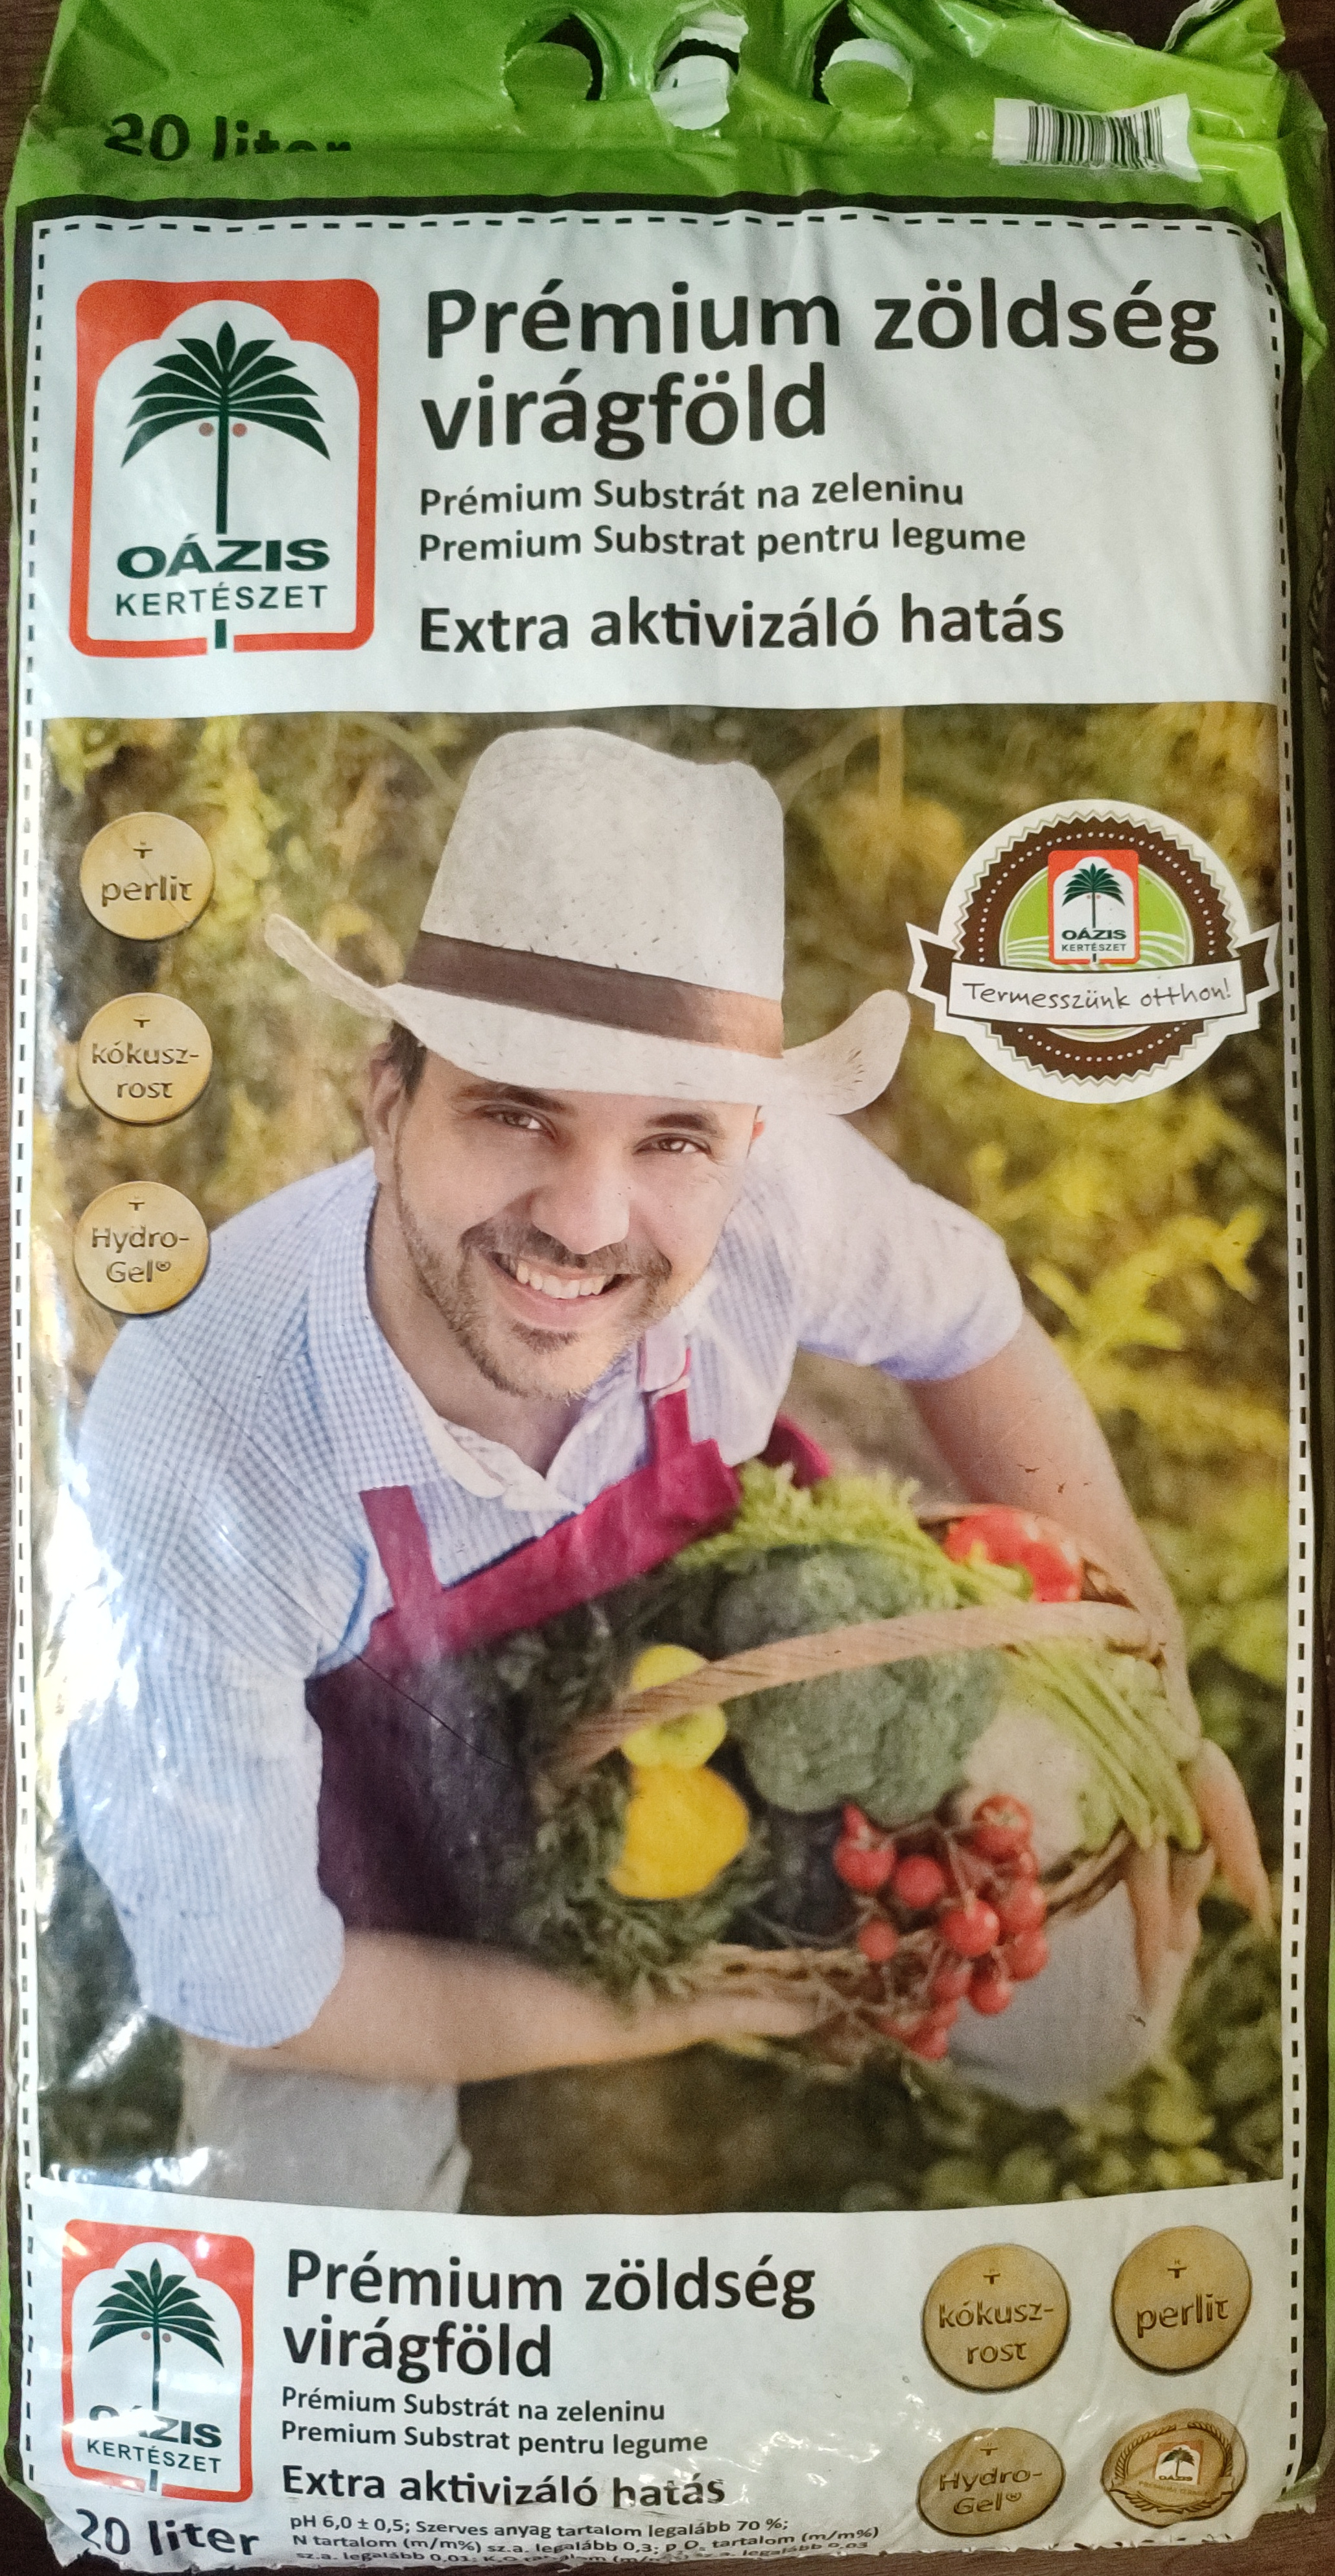
\includegraphics[width=0.5\textwidth]{assets/fertilizer_front.jpg}
	\caption{Oázis Kertészeti Kft. Premium vegetable potting soil}
	\label{fig:myimage}
\end{figure}


\begin{table}[h!]
	\centering
	\begin{tabularx}{\textwidth}{|>{\centering\arraybackslash}p{3cm}|>{\centering\arraybackslash}p{1cm}|>{\centering\arraybackslash}p{1.5cm}|>{\centering\arraybackslash}p{1.5cm}|>{\centering\arraybackslash}p{1.5cm}|>{\centering\arraybackslash}p{2cm}|>{\centering\arraybackslash}p{2cm}|}
		\hline
		Product & pH & Dry matter ($m/m\%$) & Organic matter ($m/m\%$) & Nitrogen ($m/m\%$) & Phosphorus pentoxide ($m/m\%$) & Potassium oxide ($m/m\%$) \\
		\hline
		Oázis Kertészeti Kft. Premium vegetable potting soil & 6$\pm$0,5 & $\geq30$ & $\geq70$& $\geq0,3$ & $\geq0,01$ & $\geq0,03$ \\
		\hline
	\end{tabularx}
	\caption{Chemical composition of potting soil}
	\label{tab:example}
\end{table}

The product has 4 special compound based on the description and each of them is \cite{oazis} explained by ChatGPT~\cite{chatgpt}:

\begin{itemize}
	\item \textbf{Coconut Fiber:}  
	A natural organic material that improves soil structure by enhancing aeration and water retention, promoting healthy root growth.
	
	\item \textbf{Perlite:}  
	A lightweight volcanic glass that creates a porous, airy environment in the soil, improving drainage and oxygen availability to roots.
	
	\item \textbf{HydroGel:}  
	A water-absorbing polymer that helps retain moisture in the soil, gradually releasing water to reduce the frequency of irrigation.
	
	\item \textbf{Bentonite:}  
	A type of clay mineral that acts as a nutrient reservoir, absorbing and slowly releasing nutrients, thus improving nutrient availability and preventing leaching.
\end{itemize}

Coconut fiber, perlite and bentonite are all natural compounds however HydroGel could be both synthetic or natural.











\printbibliography


\end{document}